\thispagestyle{empty}
\begin{center}
%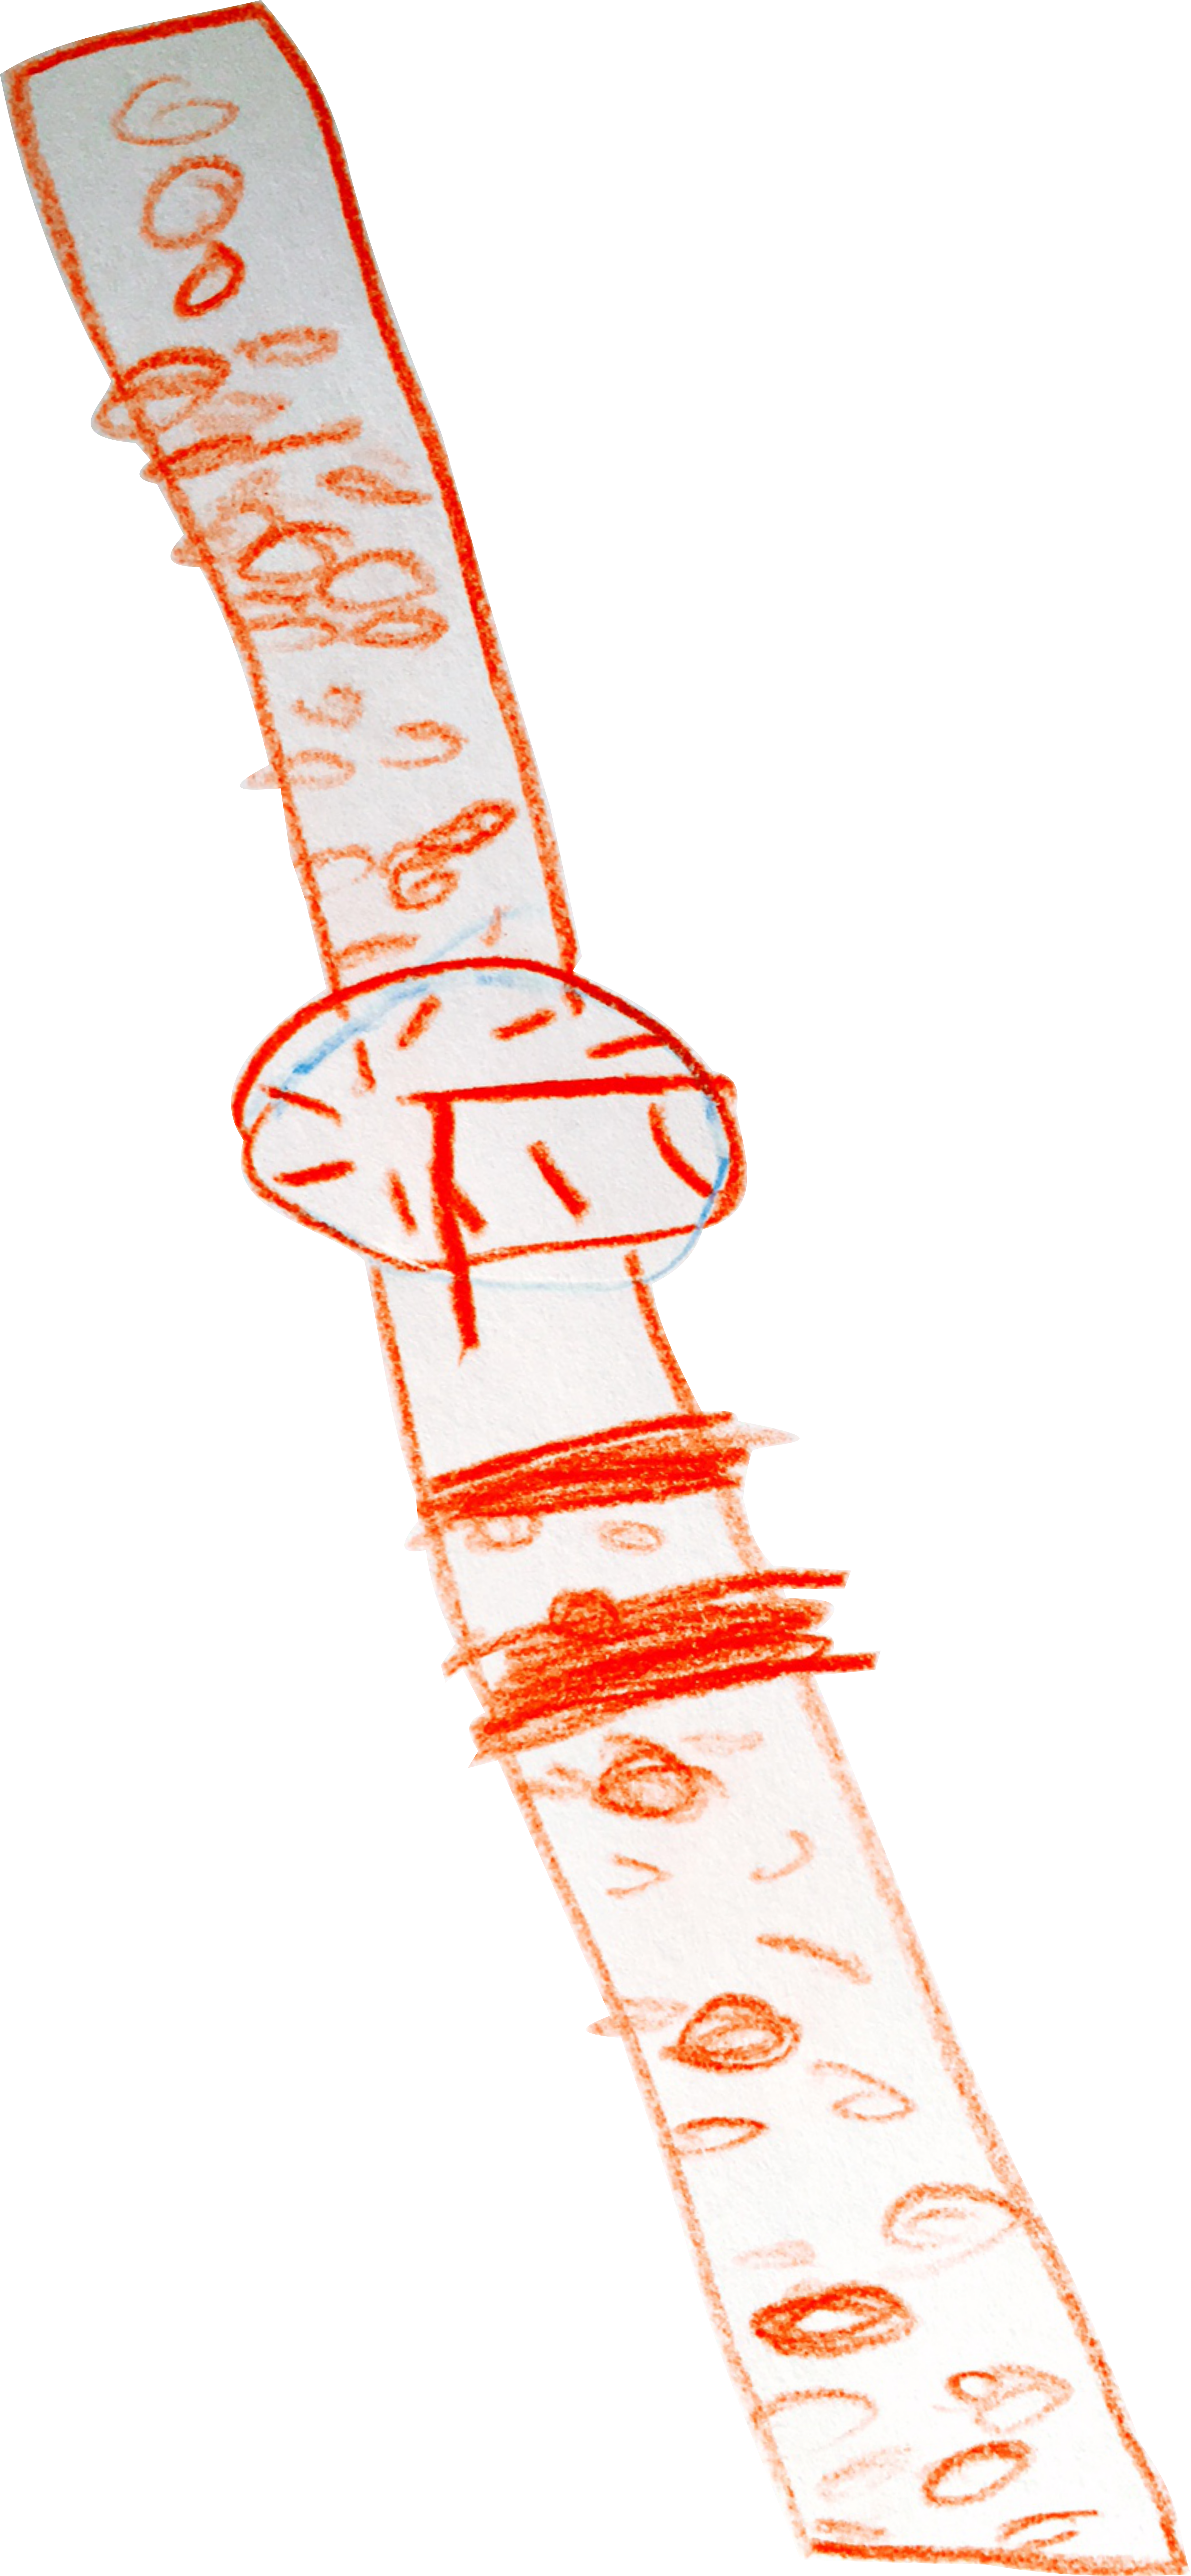
\includegraphics[height=.8\textheight]{./bilder/160120_uhr.png}
\end{center}
\vskip 2cm
{\Huge\color{farbe}\hfill{\ttfamily{Über den Staub}}}
\addcontentsline{toc}{chapter}{}
\newpage
%%%%%%%%%%%%%%%%%%%%%%%%%%%%%%%%%%%%%%%%%%%%%%%%%%%%%%%%%%%%%%%%%%%%%%%%%%%%%%%
\lettrine[lines=2, lhang=.2, loversize=.25, lraise=0.05, findent=0.1em,
nindent=0em]{M}{}aterieforscher unterscheiden verschiedene Schadklassen von Materialien. Staub gehört zur höchten Klasse, den ganzschädlichen Materialien. Eine Klasse darunter befindet sich beispielsweise Plutonium, dass zur Klasse der zweckschädlichen Materialien gehört. Die Schadklasse von Staub ist für den Wissenschaftler damit eine Höhere als Plutonium.  

Erlauben Sie mir bitte, dies als Anlass zu verstehen, der öffentlichkeit dieses Material etwas Näher zu bringen. 

Staub entsteht ganz allgemein an der Staubquelle als Nucleii. Bekannte Staubquellen sind beispielsweise Hypotrichose und andere Ursachen von Haarausfall. Staub ist daher auch mit dem Alter korreliert, woher auch der Ausdruck, etwas sei verstaubt, kommt. Der unangenehme Geruch alter Menschen hat mit deren Staubentwicklung allerdings nichts zu tun, dies ist eine mittlerweile widerlegte Hypothese. 

Eine weitere typische Staubquelle ist der Abrieb, insbesondere von Textilien. Man beobachte nur einmal den Boden einer Saune, selten wird man dort Staub entdecken können. Ein zusätzlicher Saunaeffekt ist die Bindung der Staubnucleii durch Tropfschweiss. Ganz anders ist die Situation bei Sitzmöbeln mit Textilbezug. Der Abrieb ist häufig so hoch, dass man davon ausgehen muss, dass eine durchschnittliche, zwölf Jahre alte Couch im Kern einen Staubanteil von über 80\,Prozent hat. Derartige Absitzvorichtungen bestehen daher nur sehr selten aus reinem Textil, sondern beherbergen eine Stützvorrichtung aus Metall oder Holz. Da mit steigender Summe der Besitzung der Möbel die Wahrscheinlichkeit eines Materialbruches der Stützgestänge rasant steigt, ist statische Hilfe verhärteten Staubs eine wichtige Unterstützung. Die Wahrscheinlichkeit steigt übrigens, da herausgefunden werden konnte, dass die Absitzhäufigkeit mit einer langfristigen Gewichtszunahme des Besitzenden zunimmt. Das höhere Gewicht sorgt aber wiederum für einen stärkeren Abrieb, wodurch ein gutes Möbelstück über Jahrhunderte im Gelichgewicht gehalten werden kann.

Nachdem sich jetzt Staubnucleii gebildet haben, wirken auf diese Kräfte, die eine Bewegung im Raum bewirken. Durch diese Bewegung entsteht eine statische Aufladung, die ein Zusammenballen der Nucleii zu grösseren Einheiten bewirken. Die Phase des Lebenszyklus des Staubes wird daher Transport und Akkumulation genannt. Wiet verbreitet ist der Irrglauben, Staub sei scheu und bevorzuge versteckte Ecken wie beispielsweise die Fläche unter Betten oder Schränken. Das ist lediglich ein Scheineffekt, der auf einer Scheinkraft beruht. Diese Scheinkraft bildet das grösste Rätsel der aktuellen Staubforschung. Früher hat man angenommen, dass es Luftströme sind, die Staub bewegen. Luftpakete prallen aber gerade an Objekten wie Schränken und Betten ab, Kriechströme, die auch nidere Objekte unterkriechen können, konnten bisher nicht nachgewiesen werden.

Wie also, etwas salopp formuliert, kommt der Staub dann unter das Bett? Betten heizen sich des Nachts, befeuert von der Körperwärme der Bettinsassen auf. Und Wärme ist ja nichts anderes als eine grössere Bewegung der Teilchen, was wie beschrieben zu einer grösseren Akkumulation von Staub führt. Die Staubverteilung ist üblicherweise gleichverteilt, die Akkumulationsrate hingegen nicht, weswegen der Staub unter dem Bett eher sichtbar ist, als beispielsweise im Kühlschrank.

Die Form der Staubballen folgt eigenen Gesetzen, mit denen sich ein grosser Teil der mathematischen Modullierungstheorie beschäftigt. Der interessierte Leser sein auf die Fülle entsprechender Literatur verwiesen. Eine typische Form ist die Staubwalze, wobei es wichtig ist, zwischen rechts- und linksdrehend zu unterscheiden. Sehr viel seltener die Marienform, die, wenn entstanden gerade in spanischsprachigen Ländern häufig tumultartige Reaktionen beim Staubpublikum auslöst. So manche Marienerscheinung kann durch die Staubforschung erklärt werden. Eine App zur korrekten Bestimmung der Staubform ist in Vorbereitung, bis dahin nutze man bitte die Telefon-Servicenummer.

Ein spannender Effekt hierbei ist das völlige Verschwinden jeglicher Farbpigmente der Nucleii. Staub ist immer grau und hat damit keine Farbe, wie ihnen jedes achtjährige Kind aus einer Familie, in der auf Bildung Wert gelegt wird, sagen kann. Da aber alles eine Farbe hat, ist Staub nicht! Staub gehört damit nicht zu den Dingen, sondern ist eine Materialität eigener Art, sui generis, wie wir sagen. Der Grund ist einmal mehr bei der Akkumulation zu suchen. Die dünne Schicht der Staubnucleii ist zunächst zweidimensional, räumlich also gar nicht existent. Durch Akkumulation erhöht sich diese Dimensionalität Schritt für Schritt auf einen fraktalen Wert von maximal 2.3. Dieser entspricht nebenbei bemerkt genau der Dimensionalität der Alpen! Umgangssprachlich wird diese mystische Verwandlung aus dem Nichts in etwas fast Seiendes auch als \textit{aus dem Staub erheben} bezeichnet. Dieser Gedanke ist es, den die meisten meiner Kolleginnen und Kollegen, so auch mich, Tag für Tag antreibt, sich mit dem Phänomen zu beschäftigen.

Das Ende des Lebenszyklus von Staub bildet dessen Vernichtung durch Putzen. Diese Vernichtung ist aber nur scheinbar. Tatsächlich kann Staub nur bei sehr hohen Temperaturen vernichtet werden, die lediglich im inneren von Vulkanen auf der Erde vorkommen. Ausserdem scheint es Hinweise zu geben, dass der Einstatz sehr starker Säuren einen gewissen Reduktionseffekt hervorrufen kann. Da diese aber nur mit Chemiewaffenschein erworben werden dürfen, ist keine praktische Relevanz gegeben.

Da eine Vernichtung von Staub im Hausgebrauch unmöglich ist, empfiehlt sich eine Dislotion. Im Fachhandel werden Geräte vorrätig gehalten, die sich den Horror Vacui als Grundprinzip der Natur zu Nutzen machen. Luft wird aus einem Behälter evakuiert, die entstehende Leere will sich füllen und nimmt statt der offensichtlich unzuverlässigen Luft lieber Staub. Leider erzeugt diese Leere auch immer ein lautes Geräusch, den sogenannten Schrei der Leere. Dieser wird immer als hochgradig störend empfunden, da die Leere der Natur der Welt widerspricht. Der Schrei der Leere erzeugt allgemein Wut. Beim Benutzenden des Gerätes muss der Impuls unterdrückt werden. Dies erfolgt durch einen quasireligiösen Ritus. Die zu behandelnde Fläche wird dabei vollständig abgeschritten, der Blick muss demütig in Richtung Boden gesenkt bleiben. Das funktioniert ganz unabhängig von der Benutzung der Gerätschaft, sollten sie sich also einmal dem Schrei der Leere durch ihre Nachbarn ausgesetzt fühlen, senken sie den Blick und schreiten sehr ruhig und massvoll ihre Wohnung ab, Blick immer auf die Füsse.

Der letzte Abschnitt soll die Wirkung des Staubes auf den Menschen behandeln. Staub ist als nur fats existentes Material eigentlich völlig harmlos und unschädlich. Trotzdem reagieren viele Menschen sehr intensiv auf Staub. Auch dies ist ein Phänomen, welches bisher unverstanden ist. Die Ursache scheint aber genetisch bedingt zu sein. Männer sind im Allgemeinen sehr viel weniger betroffen als Frauen und empfinden ihn erst ab sehr viel höheren Konzentrationen als störend. Alternativ zur genetischen Disposition kommen aus der Genderforschung neue Impulse, den Unterschied zu verstehen. 
\vfill
